\documentclass{article}
\usepackage[utf8]{inputenc}

\title{Assignment 1 - Data Modeling}
\author{Benny Chen}
\date{\today}

\usepackage{color}
\usepackage{amsthm}
\usepackage{amssymb} 
\usepackage{amsmath}
\usepackage{listings}
\usepackage{xcolor}
\usepackage{listings}
\usepackage{graphicx}
\usepackage[hidelinks]{hyperref}

\definecolor{codegreen}{rgb}{0,0.6,0}
\definecolor{codegray}{rgb}{0.5,0.5,0.5}
\definecolor{codepurple}{rgb}{0.58,0,0.82}
\definecolor{backcolour}{rgb}{0.95,0.95,0.92}

\lstdefinestyle{mystyle}{
    backgroundcolor=\color{backcolour},   
    commentstyle=\color{codegreen},
    keywordstyle=\color{magenta},
    numberstyle=\tiny\color{codegray},
    stringstyle=\color{codepurple},
    basicstyle=\ttfamily\footnotesize,
    breakatwhitespace=false,         
    breaklines=true,                 
    captionpos=b,                    
    keepspaces=true,                 
    numbers=left,                    
    numbersep=5pt,                  
    showspaces=false,                
    showstringspaces=false,
    showtabs=false,                  
    tabsize=2
}

\lstset{style=mystyle}

\begin{document}

\maketitle

\section*{Problem 1}

Draw an entity-relationship diagram in the space below that describes the following business environment. Use intersection data notion, not associate entities when creating the diagram. (Must include all entities, relationships, intersecting data, cardinality, and modality for full credit)

Grading Rubric: (Total 56 points)

\begin{itemize}
    \item 1 point for each = entity, attribute, relationship symbol, and unique identifier drawn out
    \item 4 points for each cardinality and modality of each relationship
    \item 2 points for intersection data symbols
\end{itemize}

\noindent\\
The Pawnee Parks \& Rec Department wants to maintain repair and maintenance logs about its sport and play structures (swing sets, benches, basketball hoops, baseball diamonds, etc), the parks and fields in which they are located, the staff they employ and the services they perform. In addition, the Department has a program by which people can be a donor of structures. The Department wants to track its donors, their dependent structures, and associated data.

\noindent\\
Each structure has a unique structure number, supplier, purchase date, maintenance instructions. Parks/Fields have a unique address, purpose, space type, and acreage. A structure can only be in one park/field. A park/field can have many structures on it or it can be currently empty. A staff member has a unique employee number, employee name, title, and year hired. Some staff supervise other staff. Staff supervisors must have staff they supervise. Every structure has been cared for by at least one and generally many staff. A staff member may not have cared for a structure, but others may have cared for many structures. Each time a staff member performs a specific, significant service for a structure the service type, date, and time are recorded.

\noindent\\
A donor donates at least one and possibly several structures. A structure may have several donors or none. A donor has a unique donor number, a name, address, and telephone number. For each exhibit that a particular donor donates, the Department wants to track the structure donor contribution and renewal date.

\begin{center}
    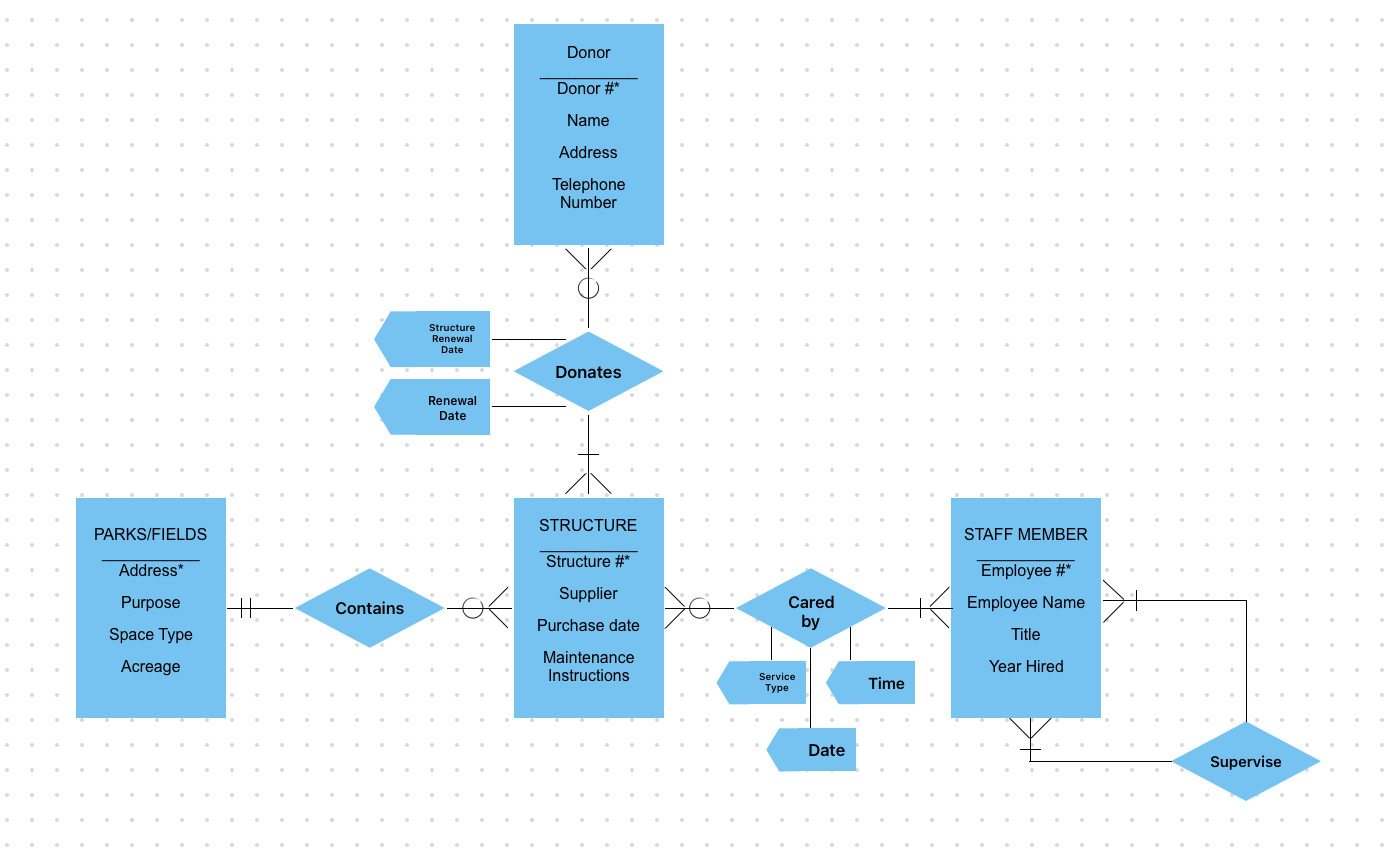
\includegraphics[width=\textwidth]{./images/Diagram.png}
\end{center}

\section*{Problem 2}
Using the following E-R Diagram write out the business environment in the space provided. (You can do this in a bulleted list in the box provided) Make sure to include intersection data and explain what type of entity that becomes in the data. (Must include all entities, unique identifiers, attributes, relationships, intersecting data, cardinality, and modality for full credit)

Grading Rubric: (Total 44 points)
\begin{itemize}
    \item 5 point for each entity with attribute and unique identifier written out
    \item 4 points for each relationship written out with cardinality and modality
    \item 2 points to write out each piece of intersection data, 4 points to write out what it becomes in the data
\end{itemize}

\noindent\\
Write out the business environment in this space provided - use bullets to break apart each entity/relationship

\begin{center}
    \noindent\rule{12cm}{0.4pt}
\end{center}

\noindent\\
From the E-R diagram, It seems that this business is trying to track the different furniture a customer would purchase along with the process of delivery.

\noindent\\
The first entity we see in the E-R diagram is the Delivery Person.

\begin{itemize}
    \item The delivery person has a unique identifier of a employee ID number
    \item They also have a driver's license number
    \item There is also data of the name, date of birth, and date of hire
\end{itemize}

\noindent\\
The second entity we see is the Furniture. 

\begin{itemize}
    \item The furniture has a unique identifier of a serial number
    \item They also have a item type to identify what type of furniture it is
    \item There is also data containg the date of purchase along with the date of delivery
\end{itemize}

\noindent\\
The third entity we see is the Customer or the Purchaser who is buying the furniture.

\begin{itemize}
    \item The customer has a unique identifier of a  username used to buy the furniture
    \item They also have the name of the customer
    \item There is also data of the email address, phone number, and address
\end{itemize}

\noindent\\
The last entity we see in this E-R diagram is the Truck which is used to deliver the furniture.

\begin{itemize}
    \item The truck has a unique identifier of a license plate number
    \item There also is the truck's make and model
    \item Lastly there is data on the truck beds dimensions or the size of the truck
\end{itemize}

\noindent\\
In this business, every entity uses Furniture. Starting from Delivery Person, there is a binary one-to-many relationship between Delivery Person and Furniture for who delivers. There is also a modality of at least one delivery person for at least zero furniture. This means that there is at least one delivery person who delivers zero to many furniture.

\noindent\\
Next, there is a binary many-to-many relationship between Purchaser to Furniture to determine purchases. There is also a modality of at least one Purchaser for at least one furniture. This means that there is at least one to many customer who purchases one to many to many furniture. There is also a intersection data to determine the date price of the purchases between the Purchaser and Furniture.

\noindent\\
Lastly, there is a binary one-to-many relationship between Furniture to Truck to determine what Furniture is assigned to which Truck. There is also a modality of at least one Truck for at least zero Furniture. This means that zero to many furniture is assigned to one truck.

\end{document}